\documentclass[12pt]{article}
\usepackage[utf8]{inputenc}
\usepackage{graphicx}
\usepackage{hyperref}
\usepackage{float}
\usepackage{pdfpages}
\usepackage{adjustbox}
\usepackage{amsmath}
\graphicspath{ {./} }
\usepackage[a4paper,width=150mm,top=25mm,bottom=25mm]{geometry}

\title{Testing Policy}
\author{Ctrl Alt Defeat}

\begin{document}
\begin{titlepage}
    \centering



    \vspace{2cm}
    \hrulefill\\
    \vspace{1cm}
    {\Huge\bfseries SRS Documentation v3.0}

    \vspace{1cm}

    {\Large Software Requirements Specification Document for\\Domain Pulse}\\
    \vspace{1cm}
    \hrulefill\\

    \vfill

    {\large Ctrl Alt Defeat}

    \vspace{1cm}

    {\large 2023/07/31}\\
    %    \vspace{1cm}
    %    \vspace{1cm}
    %    
\includegraphics[width=10cm]{../../Images/dpLogo.png}
    %    \vspace{1cm}\\
    %    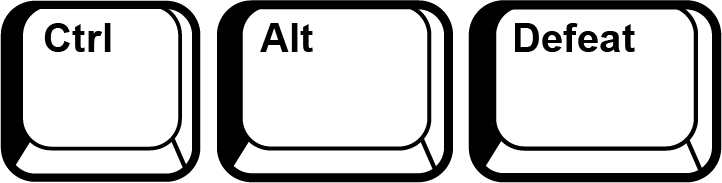
\includegraphics[width=6cm]{../../Images/cadLogo.png}

\end{titlepage}


\tableofcontents
\newpage

\newpage
\section{Quality Requirements Testing}
\subsection{Usability}
\subsubsection{Process of Usability Testing}
\begin{itemize}
    \item \textbf{Planning} - The first step in usability testing is to plan what you want to test and how you are going to test it.
    \item \textbf{Recruiting} - The next step is to recruit participants to test the application. The participants should be representative of the target audience of the application but should also be diverse enough to get a wide range of feedback.
    \item \textbf{Testing} - The next step is the actual testing of the application, the way in which we facilitated the testing of the application was as follows:
          \begin{itemize}
              \item We sent all participants of our usability testing a pdf explaining all aspects of navigating to the app and a list of tasks in which they could try. The pdf can be found \href{https://github.com/COS301-SE-2023/Domain-Pulse-A-Sentiment-Analysis-Platform/blob/docs/Demo4Documentation/documentation/Testing%20Policy/Testing_Assistance_Domain_Pulse.pdf}{HERE.}
              \item The participant will access the application in their own time in the environment of their liking and use the application to perform tasks that were suggested on the pdf.
              \item Once the user has completed the testing of the app, a questionnaire was then to be filled out by all participants, the questionnaire can be found \href{https://forms.gle/P6EC4iyg7ZD93LNfA}{HERE.}
          \end{itemize}
    \item \textbf{Feedback implementation} - We collect all data from the questionnaire that the testing participants filled out and use this to modify and fix issues accordingly.
\end{itemize}

\subsubsection{Metrics, requirements and results for usability testing}
The metrics that we used to measure the usability of our application are the following:

\begin{itemize}
    \item \textbf{How insightful the application is} which is computed as an average with 1 being the least insightful and 10 being the most insightful. Our minimum requirement for this metric was a score of 8/10 - this benchmark was exceed with a score of 8.76. As demonstrated in the below graph image below the majority of the users we tested rated the insightfulness of the applications statistics as an 8 or higher.
          \begin{figure}[H]
              \centering
              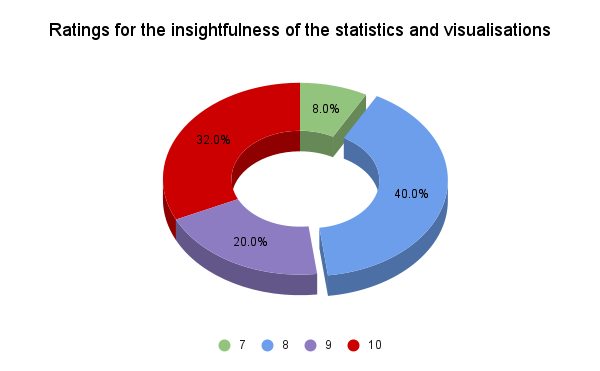
\includegraphics[width=0.9\textwidth]{piechart.png}
          \end{figure}
    \item \textbf{The overall rating of the application} which is computed as an average with 1 being the weakest rating and 10 being the strongest rating. Our minimum requirement for this score was a score of 8/10 - this benchmark was exceeded with a score of 8.48. Furthermore, users over the age of 40 the overall app as a 8.375 on average while users under the age of 40 on average rated the overall app as a 8.647 - indicating that this metric remained fairly consistent across age ranges. As we can see from the image below, the majority of users rated the application 8 or higher.
          \begin{figure}[H]
              \centering
              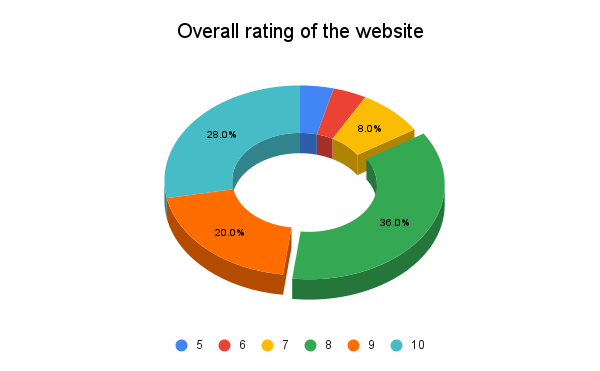
\includegraphics[width=0.9\textwidth]{Overall rating of the website.png}
          \end{figure}
    \item \textbf{The number of responses regarding how easy the website is to use and navigate} ranging from very easy to very difficult. As we can see the majority of users rated the app as easy to very easy to use.
          \begin{figure}[H]
              \centering
              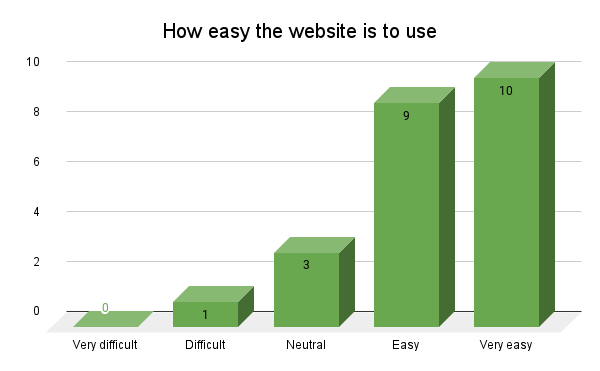
\includegraphics[width=0.9\textwidth]{How easy the website is to use.png}
          \end{figure}
    \item \textbf{The overall sentiment of the responses regarding the application.} Having developed our own Sentiment Analysis Platform, we fed the user reviews obtained through testing into Domain Pulse's engine by means of a CSV file, such to obtain an understanding of the overarching sentiment the testers had toward the application! Our minimum requirements for this metric are an overall score of 75\% with 'joy' being the most dominant emotion. The results of the sentiment analysis can be found in the below report, which was generated by our Domain Pulse. After running the results of the usability testing through our application, some very valuable insights were apparent which can be seen in the pdf above. We can see from the generated insights that we have an \textbf{overall score of 87\%} (exceeding expectations) which is great and shows that our application is user friendly and easy to use with a minimal learning curve. When the designers were designing the user interface we wanted to promote recognition over recall which allows the user of the application to easily identify and select the actions they want to complete, rather than having to remember the UI and all its functionality. The main emotion that was felt when using our app \textbf{was indeed joy, with a very dominant score coming in at 76\%} which shows that users had a pleasant experience when using our application. We believe this is due to the fact that the app was designed in a way that is intuitive and can be used by people from most technological backgrounds and age, With many support aids available to help users navigate the application such as tooltips and help buttons. The sentiment ratios that were generated by our application for the usability testing responses were as follows:
          \begin{itemize}
              \item Positive - 52\%
              \item Negative - 10\%
              \item Neutral - 36\%
              \item Undecided - 2\%
          \end{itemize}
          The sentiment ratios again reiterate the fact that the majority of users had a pleasant experience when using our application.
          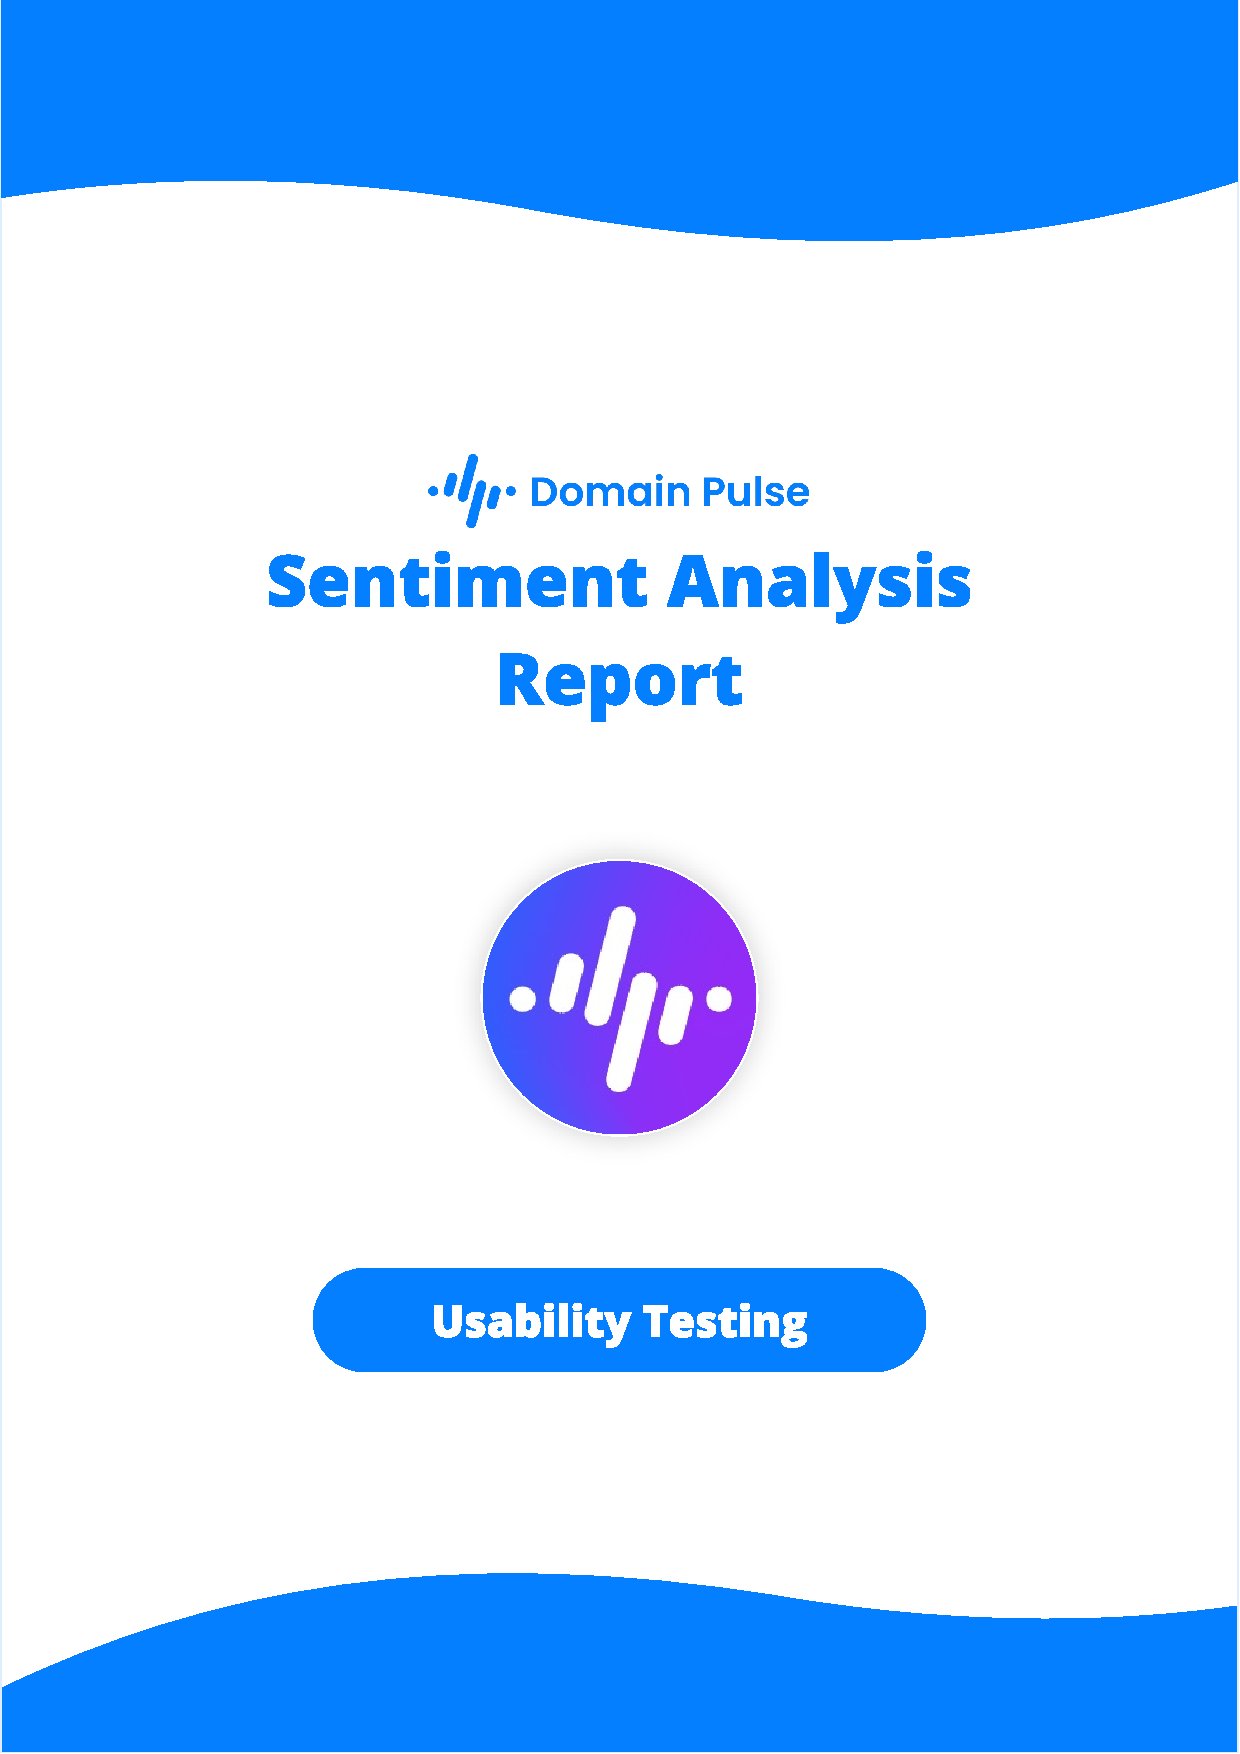
\includepdf[pages=-]{UTR.pdf}

    \item \textbf{The number of clicks required to complete any action} within the app should be 5 or fewer clicks (from the data dashboard page).
          % \begin{figure}[H]
          %     \centering
          %     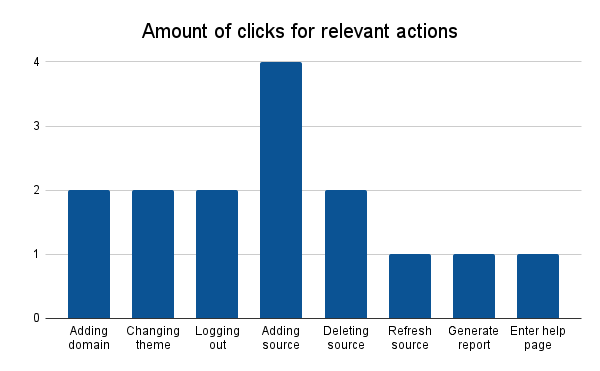
\includegraphics[width=0.9\textwidth]{Amount of clicks for relevant actions-2.png}
          % \end{figure}
          \begin{figure}[H]
              \centering
              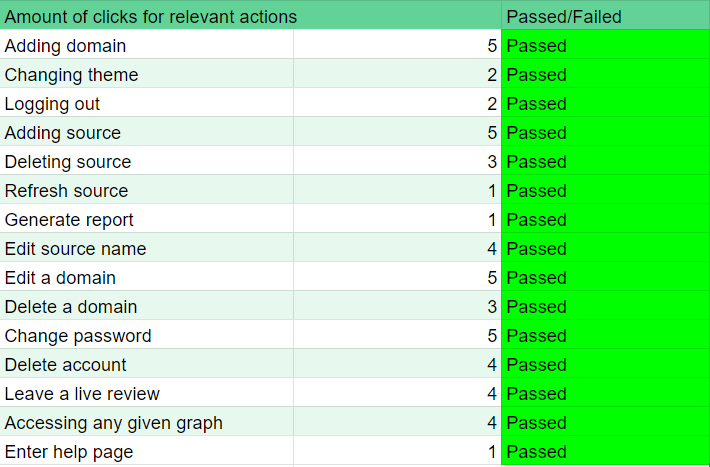
\includegraphics[width=0.9\textwidth]{table2.png}
          \end{figure}
\end{itemize}

\subsubsection{Other issues}
The results of our usability testing gave view to many insights and helpful information regarding our application. Some prominent information that the usability testing brought to light was the bugs within our application that needed to be rectified and the consequences of not fixing bugs within the application.
A list to some of the bigger bugs has been supplied below:
\begin{itemize}
    \item The App was not redirecting to the login page after registering a new user.
    \item The headings for the relevant input fields were not displaying correctly.
    \item Forgot password functionality was not working properly.
    \item Scanning our live review source on an android device takes the user to the notes app instead of our modal for user input data.
    \item Live review loads indefinitely when there is no data.
    \item Live data would display with incorrect timestamps
    \item Occasional, unexpected errors when performing CRUD operations on domains and sources
\end{itemize}
All the aforementioned bugs (and a host more) have been fixed suh that Domain Pulse is in a state that is bug free to our knowledge.
\\
Improvements within the app also came to light during the usability testing and these improvements have been implemented and are as follows:
\begin{itemize}
    \item Wider scroll bars were added to aid those with visual impairments.
    \item Improved help page wording.
    \item Improved colour pallette for badges, text, and icons.
    \item The ability to toggle a users password visibility was added.
    \item Clearer graph switching buttons were added.
    \item Filtering of comments were added to allow users to search for comments.
    \item Adjustable sample data pane.
\end{itemize}

Ultimately the usability quality requirement was met and exceeded by our application and we are very proud of the results that were achieved.


\newpage
% \subsection{Availability}
% Availability refers to the probability of a system functioning as intended when desired. Availability is important within our system due to the
% necessity of the live review service to be available whenever a user requires it.
% \subsubsection{Quantification}
% Domain Pulse uses Microsoft Azure App Service for hosting and therefore availability is highly reliant on the availability of the Azure App Service.
% As well as this, Domain Pulse, hosts a PostgreSQL database and several MongoDB databases on private servers. The availability of these databases
% is highly improved by redundancy across several servers, with quick switch-over time, allowing for little to no downtime should a database fail.
% A total Availability of 99.5\% per month will be the minimum requirement for the system to be considered acceptably available, whereby
% availability is calculated as follows:
% \begin{equation}
%     Availability = \frac{Uptime}{Uptime + Downtime} * 100
% \end{equation}

% \subsubsection{Results}
% Microsoft Azure App Service calculates the Uptime Percentage, which is practically the same metric as Availability, using the equation
% \begin{equation}
%     \frac{Maximum Available Minutes-Downtime}{Maximum Available Minutes} * 100
% \end{equation}
% , where Maximum Available Minutes is the total minutes in a billing month, and Maximum Available Minutes-Downtime is the total number of minutes that the app was unavailable during the billing month.
% Within the SLA (Service Level Agreement), an Uptime Percentage of less than 99.95\% results in a credit refund of 10\%, an uptime of less than 99\%, results in a credit refund of 25\%, and an uptime of less than 95\%, resulting in a full refund.
% This promise of credit refund, shows a high level of confidence in the availability of the Azure App Service, and therefore the availability of Domain Pulse, being higher than 99.95\%.

\newpage
\subsection{Security}
Security is a very important quality requirement for any application as peoples information is at risk if the application is not secure. The security of our application is of utmost importance as we are dealing with peoples personal information and we need to ensure that this information is kept safe and secure. The security of our application in relation to the OWASP top 10 security vulnerabilities is as follows:
\begin{itemize}
    \item \textbf{Broken access control} - We are using Django's support for user authentication which has been thoroughly tested and is highly secure, with this being said access control is very unlikely to be broken unless one of Django's authentication libraries had a flaw which is unlikely. Our application only have 1 level of access which means that incorrect access control is unlikely to occur.
    \item \textbf{Cryptographic failures} - To protect our system against cryptographic failures we are using HTTPS and for all our password storage we are using state of the art hashing with salting.
    \item \textbf{Injection} - To protect our system against injection attacks we are using prepared statements provided by Django's built in ORM (Object Relational Mapper) which is highly secure and has been thoroughly tested. We also use built in functions to execute our queries to ensure that no injection attacks can occur.
    \item \textbf{Insecure design} - We consistently update the architecture of our system which allowed us to identify and fix any insecure design flaws that may have been present in our system.
    \item \textbf{Security misconfiguration} - We have tested our application extensively and have ensured that the way our security configurations work is correct and secure.
    \item \textbf{Vulnerable and outdated components} - We have a bot that updates our dependencies automatically and we have no known vulnerabilities in our dependencies, we also make use of Gitguardian which alerts us if any secrets within the repo somehow get leaked.
    \item \textbf{Identification and Authentication failure} - Once again we use Django's built lt in authentication libraries which have been thoroughly tested and are highly secure.
    \item \textbf{Software and data integrity failure} - All libraries and plugins that are used within our system are from trusted sources and hence we can be sure that there are no integrity failures that are known to us.
    \item \textbf{Security logging and monitoring failure} - We use software(Fail2ban) that bans an IP address from accessing our VM if more than 3 attempts to access the Vm are made and failed.
    \item \textbf{Server-side request forgery} - We only allow users to choose from sources that the application trusts and hence don't allow the user to make requests to any other sources which restricts the range of allowed URLs that can be used as input by the user. Another added measure that we have incorporated is URL validation which ensures the user is only allowed to use URLs that are valid.
\end{itemize}
\newpage
\subsection{Performance}
Performance is a highly important quality requirement within our application. This is due to the large amount of data processing that is done by our application, and therefore, the requirement of the reported data being consistent, accurate and computed in a reasonable amount of time.
\subsubsection{Quantification}
The following metrics are used to quantify the performance of the system, being the most important metrics to the system:
\begin{itemize}
    \item \textbf{Response Time} - The time taken for the system to respond to a request, being the time taken for the system to process the request and return a response. This is of importance due to the need for data to be returned in a reasonable amount of time, heavily relating to the usability of the system.
          The metric used shall be the average response time of several frequently used requests, and comparing these results to a list of minimum requirements for each endpoint.
    \item \textbf{Accuracy and Consistency} - The accuracy and consistency of the Sentiment Analysis models used within the system are of utmost importance, such that a user receives relevant data that provides useful and precise information regarding their domains, that is consistent with in multiple requests.
          As the models used are pre-trained, the accuracy can be determined by their reported accuracy, and F1-score. Accuracy within a model refers to percentage of correct predictions made on a class-balanced dataset (datasets with the same number of samples), while we often have varying dataset sizes, and therefore F1 score is a better metric and shall be used. As reviewing the statistical accuracy of each model, the accuracy shall be tested by providing highly positive and highly negative test data to the system, and reporting on the results.
\end{itemize}

\subsubsection{Results}
The following results have been collected from the system, and are used to determine the performance of the system:
\begin{itemize}
    \item \textbf{Response Time} - The endpoints create\_domain, refresh\_source (which is calculated from the summation of its initial call and subsequent calls for real-time data loading), generate\_report, login\_user, get\_domain\_dashboard and get\_source\_dashboard have been tested on sample data (of which has contained the same data for fair results), and the average response times have been measured as such:
          \begin{figure}[H]
              \centering
              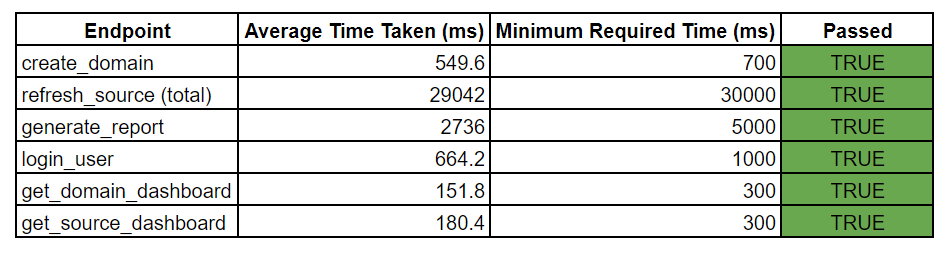
\includegraphics[width=0.9\textwidth]{PerfTable.png}
          \end{figure}
          According to Google (https://developers.google.com/speed/docs/insights/Server), the response time of your server should be under 200 ms. Response times of under 200ms will provide users with, what feels like an instantaneous response. Therefore the minimum response times of endpoints used within navigation of the website, such as get\_domain\_dashboard and get\_source\_dashboard, should be under 300 ms, so as to accommodate for large amounts of data being parsed throughout the application.
          The minimum requirement of the response time for generate\_report and refresh\_source are 5000 ms and 30000 ms respectively, this is due to the large amount of data processing required in each of these endpoints, and therefore, the time taken to process the data is expected to be longer. This performance, however, does not negatively impact user experience as data will be loaded into the dashboard whilst further data is being processed, and the processing of data is expected to take a longer amount of time.
          Similarly create\_domain has a minimum requirement of 700 ms due to the necessity of creation of data. The login\_user endpoint has a requirement of 1000 ms to accommodate for authentication to be completed.
    \item \textbf{Accuracy and Consistency} - The accuracy and consistency of each model is tested by their accuracy, F1 score, and differences within the resulting data after testing the same source.
          The consistency of the models has been tested by rerunning the same analysis on the same source, 10 times, twice, whereby every result for the each source respectively is identical.
          The accuracy of the models is determined by the metrics provided by the authors of the models, being the accuracy and F1 score, which are as follows for each model:
    \item \textbf{VADER} - The VADER model is found to have a F1 score of 0.96, which is extremely high and extremely accurate, therefore contributing to high performing data analysis within our system.
    \item \textbf{DistilBERT base uncased finetuned SST-2} This general model is used alongside the VADER model to calculate the general sentiment score of the given data. The reported accuracy of the model is as such:
          \begin{figure}[H]
              \centering
              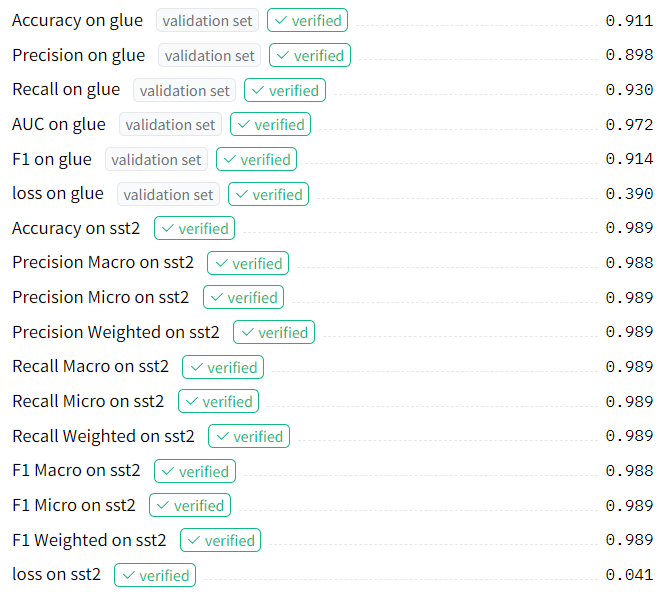
\includegraphics[width=0.9\textwidth]{GeneralAccuracy.png}
          \end{figure}
          These findings lead to a resultant average accuracy of 0.95, and a resultant average F1 score of 0.9515 which is an exceptionally high F1 score, and therefore, leading to highly accurate data analysis and information in our system.

    \item \textbf{DistilBERT toxic-comment-model} This model is used to calculate the toxicity of a single comment, and therefore is a less significant statistic within our system, however, the accuracy of the model is still of importance. The reported accuracy of the model is an Accuracy of 94\%, and a F1-score of 0.59, which although is a slightly above average score, is not detrimental to our systems integrity, as toxicity is not a highly important statistic for our system or for users viewing it.
    \item \textbf{emotion-english-distilroberta-base} This model is used to calculate the prevalent emotions within a review. The reported accuracy of the model is an Accuracy of 66\% which is relatively performant, due to the difficulty in detection of emotion within toneless text, and a share/spread of different emotion within a review.
    \item \textbf{Polarized Data} As stated in the Quantification, highly, objectively, positive and negative data sources were parsed into the system, and the results were as follows:
          \begin{figure}[H]
              \centering
              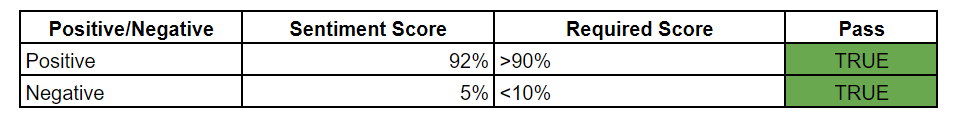
\includegraphics[width=0.9\textwidth]{PositiveAndNegative.png}
          \end{figure}
          The results of the polarized data show that the system performs to the desired standard, and will provide consistent, accurate data to the user.
\end{itemize}
\newpage
\subsection{Scalability}
Scalability refers to the capability for our system to work under heavier loads. It's imperative for our system to be sufficiently scalable as large numbers of users shall be making requests, resulting in a large number of heavy data processing, which should not heavily effect the performance and furthermore, usability of the system.

\subsubsection{Quantification}
The following metrics are used to quantify the scalability of the system.
\begin{itemize}
    \item \textbf{Load Tested Response Time} - Similarly to testing response time in the testing of performance, we will measure the average time taken for the system to respond to main requests made within the system. However, unlike our performance testing, we will be testing these endpoints under many different loads, such as while processing 50, 100 or 1000 concurrent requests.
          The way in which we will achieve this is by sending varying numbers of concurrent reviews to a live source, and measuring the response time of each request. These results need to have a maximum response time, under the minimum requirement.
          The required time will be calculated using an equation:
          \begin{equation}
              \begin{aligned}
                   & y=x^{1.6}+1600               \\
                   & x= Number\:of\:Data\:Entries \\
                   & y= Time\:taken\:(ms)         \\
              \end{aligned}
          \end{equation}
\end{itemize}
\subsubsection{Results}
The following results have been collected from the system, and are used to determine the scalability of the system:
\begin{figure}[H]
    \centering
    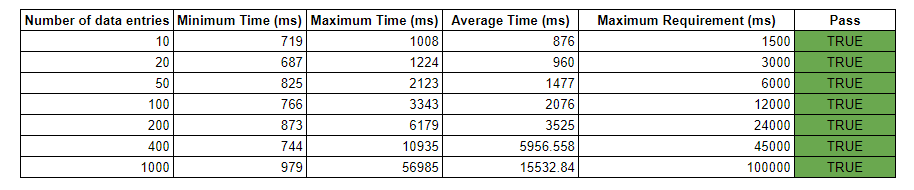
\includegraphics[width=0.9\textwidth]{Scalability.png}
\end{figure}
\begin{figure}[H]
    \centering
    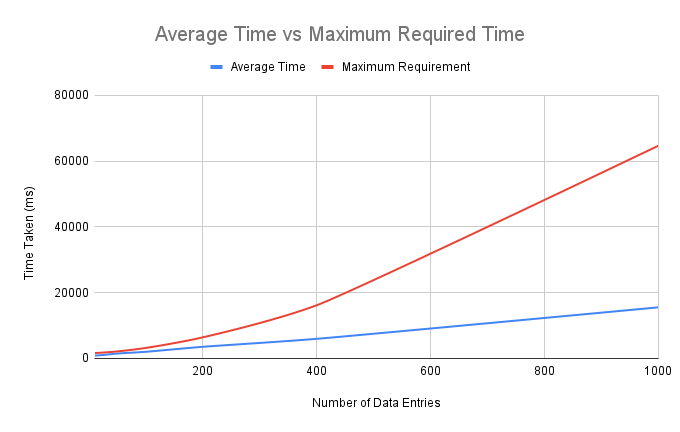
\includegraphics[width=0.9\textwidth]{Average Time vs Maximum Required Time.png}
\end{figure}
\begin{figure}[H]
    \centering
    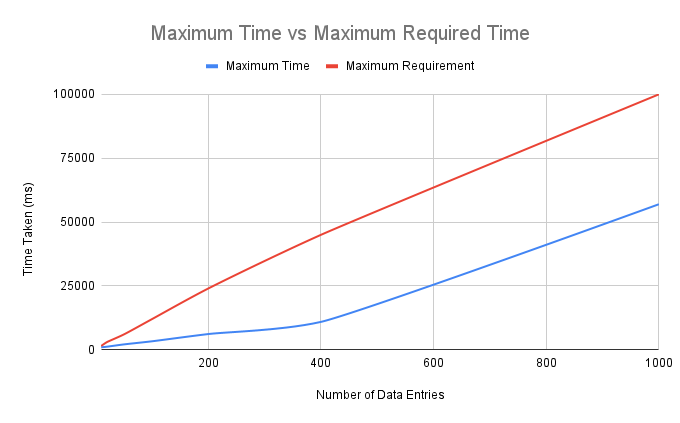
\includegraphics[width=0.9\textwidth]{Maximum Time vs Maximum Required Time.png}
\end{figure}
It is clear from the above graphs that the system is sufficiently scalable, as the average response time of the system is well below the requirement, and the maximum response time is also below the requirement, with the gradient of maximum response time and the requirement being similar, and increasing at a similar rate.

\newpage
\subsection{Modifiability}
Modifiability is an important quality requirement within our project, due to the need for multiple services that perform semi-independent functions, and the need for these services to be easily maintained and extensible.
\subsubsection{Quantification}
The metric used to quantify the Modifiability of the system will be the Maintainability index and Cyclomatic Complexity values. Cyclomatic Complexity refers to the complexity of a program and uses the number of linearly-independent paths through a program module to determine how risky, understandable and simple to modify a codebase is, where the equation is:
\begin{equation}
    \begin{aligned}
         & M = E - N + 2P                                    \\
         & N = the number of nodes in the control flow graph \\
         & P = the number of connected components
    \end{aligned}
\end{equation}
The Maintainability index is a scale from 0 to 100, with 100 being the most maintainable, and 0 being the least maintainable. The Maintainability index is calculated using the following equation:
\begin{equation}
    \begin{aligned}
         & MI = MAX(0, (171 - 5.2 * ln(Halstead Volume) \\
         & - 0.23 * (Cyclomatic Complexity)             \\
         & - 16.2 * ln(Lines of Code)) * 100 / 171)
    \end{aligned}
\end{equation}
Where Halstead Volume is calculated with:
\begin{equation}
    \begin{aligned}
         & Volume = N * log_2(n)                         \\
         & N = Total number of operators and operands    \\
         & n = Number of distinct operators and operands
    \end{aligned}
\end{equation}
Within the Maintainability index, a score above 20 is considered a good Maintainability index, and a score below 10 is considered a poor Maintainability index.
Within Cyclomatic Complexity, a score below 4 is considered good (simple), while a score above 7 is considered bad (complex).

\subsubsection{Results}
Due to the complexity of our system, and near all computations within our system, being performed by the backend, the results are based on the backend of our system, to exclude unimportant information.
The results, for each service within our system are as follows:
\begin{figure}[H]
    \centering
    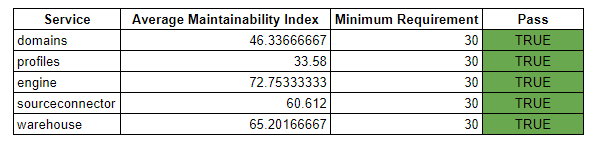
\includegraphics[width=0.9\textwidth]{Maintainability.png}
\end{figure}
A Maintainability index of 30 is considered the minimum requirement, as it is considered higher than the minimum 'good' index, and our system needs a high level of extensibility and simplicity within the codebase.
\begin{figure}[H]
    \centering
    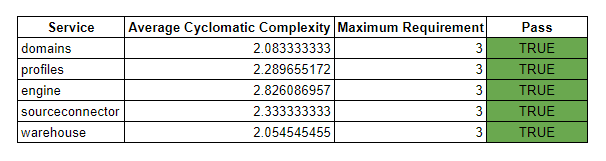
\includegraphics[width=0.9\textwidth]{Cyclomatic.png}
\end{figure}
Similarly to the minimum Maintainability index value, 3 is considered the maximum value for our Cyclomatic Complexity to ensure a simple and readable codebase, for ease of development.
\\\\Therefore all tests have passed, and the system is considered to be highly modifiable.
\newpage
\section{Code Coverage}
Any commit made to a branch causes automated tests to be run on the codebase of that branch, thereafter the code coverage of said branch is calculated.
Any branch being merged via pull request into the development branch (dev) needs to have the coverage of changes to the codebase to match or better the coverage of the development branch.
\\\\Furthermore, the coverage of the newly committed code (ie: patch) must match or exceed the coverage percentage of the project.
This ensures that the coverage of the codebase is never decreasing, and that sufficient testing is being done on the codebase.
Furthermore any time the development branch is merged into the master branch, the coverage of the development branch must match or be higher than that of the master branch, ensuring an increasing coverage and sufficient testing.
\begin{itemize}
    \item A code coverage report is included in the below image:
    \item A link to our code cov profile can be found \href{https://codecov.io/gh/COS301-SE-2023/Domain-Pulse-A-Sentiment-Analysis-Platform}{HERE.}
\end{itemize}
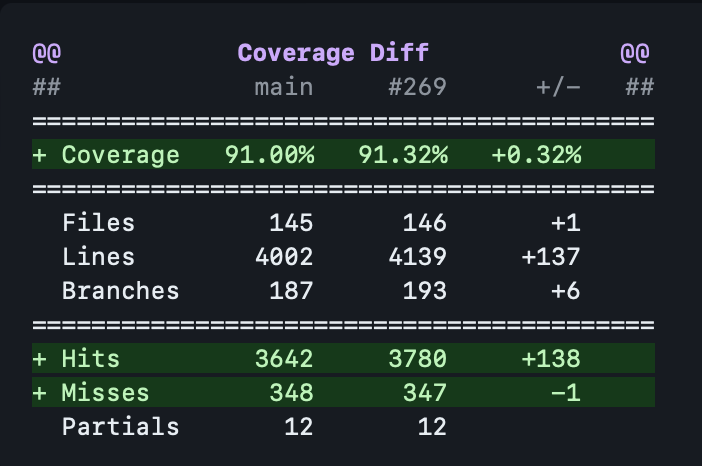
\includegraphics{codecovReport.png}

\newpage
\section{Types of testing}
\begin{itemize}
    \item \textbf{Unit testing} - Unit testing is when the smallest parts of the application which are known as units are tested to ensure that the correct operation occurs. An example of Unit tests and integration tests can be found in any file ending in "spec.ts" for frontend and an example is given \href {https://github.com/COS301-SE-2023/Domain-Pulse-A-Sentiment-Analysis-Platform/blob/dev/frontend/src/app/main/main.component.spec.ts}{HERE} and a backend example can be found \href {https://github.com/COS301-SE-2023/Domain-Pulse-A-Sentiment-Analysis-Platform/blob/main/backend/engine/analyser/tests.py}{HERE.}
    \item \textbf{Integration Testing} - Integration testing is when separate components are tested together to ensure the correct operation of these components occur. Integration tests can be mocked or un-mocked, mocked tests are when the data used in the tests are not pulled in from an external API or database but rather mocked data is used to simulate the data that would be pulled in from an external API or database. Unmocked tests are when the data used in the tests are pulled in from an external API or database.
    \item \textbf{E2E Testing} - End to end testing is when the application is tested as a whole to ensure that the application is working as expected from the user interface level all the way through the application to the database level and checks all the integration between these components work as expected. Examples of E2E tests can be found in any file ending in a ".cy.ts" for frontend and an example is given \href {https://github.com/COS301-SE-2023/Domain-Pulse-A-Sentiment-Analysis-Platform/blob/main/frontend/cypress/e2e/accountsManage.cy.ts}{HERE.}
\end{itemize}
\newpage
\section{Choice of testing tools/frameworks}
\subsection{Frontend Testing}
For our frontend testing frameworks and tools we decided to use the following:
\begin{itemize}
    \item \textbf{Karma and Jasmine} - Jasmine is the testing framework that is used to write actual tests and are typed in Javascript, Karma is the test runner that executes the tests. Karma is run from a CLI(Command Line Interface) and it will open up a browser window and run the tests in that browser. Karma will then report the results of the tests back to the CLI and can be used to generate a coverage report. Karma and Jasmine are recommended by Angular which is what our frontend is primarily built upon and they are the most popular testing frameworks for Angular applications. The advantages of using Karma and Jasmine over other testing frameworks is that they are easy to set up and use, they are well documented and they are popular amongst Angular developers which means there is a extensive amount of resources available online for help if need be.
    \item \textbf{Cypress} - Cypress is a testing framework that is used to write end to end tests which are tests that try and simulate a user using the application. End to end tests are needed to ensure that the application is working exactly as expected from the user interface level all the way through the application to the database level and checks all the integration between these components work as expected. Cypress runs in a browser which makes it easy to setup and follow the tests as they execute in the browser. Cypress is documented well with a thriving community which allows for easy access to information if any problems arise.
\end{itemize}

\subsection{Backend Testing}
For our backend testing framework and tools we decided to use the following:
\begin{itemize}
    \item \textbf{Django built in testing module} - Django has a built in testing module which allows for the testing of Django applications, this is yet another reason why we decided to use django as it has amazing functionality out of the box. The django testing module allows for extensive testing of the application. The advantages of using django testing framework over an external framework is that one is already used to the syntax of django since our backend is primarily built on django and hence saves valuable time trying to learn syntax of another backend testing framework. Django allows for fast pace development which is much needed in certain situations such as in ours when following an agile development strategy. Django testing framework is also well documented and has a large community which allows for easy access to information if any problems arise and help is needed.
\end{itemize}

\subsection{Github Actions and workflows}
Github actions were used to aid in the automatic testing and generating of code coverage reports for our application. Github actions are workflows that are activated by certain events such as a merge, push or pull to certain branches of the repository. The workflows are defined in a yaml file and are run on a virtual machine hosted by github, Github actions ensure that all tests pass before a branch is merged into main/master. The workflows that we have defined are as follows:
\begin{itemize}
    \item backend build
    \item frontend build
    \item coverage report
    \item automatic deployment
    \item automatic testing
\end{itemize}

\end{document}